\documentclass{article}

\usepackage[usenames,dvipsnames]{color}
\usepackage{bm}
\usepackage{amsmath}
\usepackage{amssymb}
\usepackage{graphicx}
\usepackage[colorlinks=true,urlcolor=blue]{hyperref}
\usepackage{geometry}
\geometry{margin=1in}
\usepackage{float}
\setlength{\marginparwidth}{2.15cm}
\usepackage{booktabs}
\usepackage{epsfig}
\usepackage{setspace}
\usepackage{parskip}
\usepackage[]{algorithm2e}
\usepackage{comment}
\usepackage{pdfpages}
%\usepackage{physics}
\usepackage{enumerate}

%\newcommand{\comment}[1]{\textcolor{blue}{\textsc{\textbf{[#1]}}}}

 \newenvironment{soln}{
     \leavevmode\color{blue}\ignorespaces
 }{}

\makeatletter
\newcommand{\removelatexerror}{\let\@latex@error\@gobble}
\makeatother

\begin{document}

\section*{}
\begin{center}
  \centerline{\textsc{\LARGE Homework 1}}
  \vspace{0.5em}
  \centerline{\textsc{\Large MLE, MAP estimates; Linear and Logistic Regression}}
  \vspace{1em}
  \textsc{\large CMU 10-701: Machine Learning (Spring 2017)} \\
  \vspace{1em}
  \centerline{OUT: Jan 31}
  \centerline{DUE: Feb 10, 11:59 PM}
  \centerline{NAME: Mengwen He}
  \centerline{ADREW ID: mengwenh}
	
\end{center}

\section*{Part A: Multiple Choice Questions}

\begin{enumerate}
	\item For each case listed below, what type of machine learning problem does it belong to?
	\begin{enumerate}
		\item Advertisement selection system, which can predict the probability whether a customer will click on an ad or not based on the search history. \\
		\textbf{Answer:}
		\underline{B. Supervised learning: Regression}\\
		A task, with ads click statistics and search history as input data, outputs the prediction of continuous probability of clicking an ad.
		\item U.S post offices use a system to automatically recognize handwriting on the envelope. \\
		\textbf{Answer:}
		\underline{A. Supervised learning: Classification}\\
		A task, with handwriting samples and their labels as input data, outputs the prediction of discrete numbers/letters of a handwriting on the envelope.
		\item Reduce dimensionality using principal components analysis (PCA). \\
		\textbf{Answer:}
		\underline{C. Unsupervised learning}\\
		A task, without training data as input, outputs a description of reduced dimensionality. 
		\item Trading companies try to predict future stock market based on current market conditions. \\
		\textbf{Answer:}
		\begin{itemize}
			\item \underline{A. Supervised learning: Classification}\\
			A task, with current market conditions as input, outputs the prediction of discrete stock market conditions, say bull or bear market.
			\item \underline{B. Supervised learning: Regression}\\
			A task, with current market conditions as input, outputs the prediction of continuous stock market conditions, say stock price.
		\end{itemize}
		
		\item Repair a digital image that has been partially damaged. \\
		\textbf{Answer:}
		\begin{itemize}
			\item \underline{A. Supervised learning: Classification}\\
			A task, with digital images database as input, outputs the prediction of discrete pixel value in the damaged zone.
			\item \underline{B. Supervised learning: Regression}\\
			A task, with digital images database as input, outputs the prediction of continuous parameters of a color distribution model to form a discrete patch to cover the damaged zone.
			\item \underline{C. Unsupervised learning}\\
			A task, without training data as input, outputs a description of a damaged pixel according to its surrounding pixel values, e.g. interpolation or extrapolation.
		\end{itemize}
	\end{enumerate}
	Type of machine learning problem:
	\begin{itemize}
		\item [A.] Supervised learning: Classification
		\item [B.] Supervised learning: Regression
		\item [C.] Unsupervised learning
	\end{itemize}
	
	\item For four statements below, which one is wrong?
	\begin{itemize}
		\item [A.] In maximum a posterior (MAP) estimate, data overwhelms the prior if we have enough data.
		\item [B.] There are no parameters in non-parametirc models.
		\item [C.] $P(X \cap Y \cap Z)=P(Z|X \cap Y) P(Y|X) P(X)$.
		\item [D.] Compared with parametric models, non-parameter models are flexible, since they don't make strong assumptions.
	\end{itemize}
	\textbf{Answer:}
	\underline{B. There are no parameters in non-parametirc models.} is wrong.\\
	Non-parametric model still needs parameters to describe the model, but the number of model's parameters is not fixed and will grow with the data size. The non-parametric only means that there is weak assumption on the model's type defined by a fixed number of parameters.
	
	\item There are about $12\%$ people in U.S. having breast cancer during their lifetime. One patient has a positive result for the medical test. Suppose the sensitivity of this test is $90\%$, meaning the test will be positive with probability $0.9$ if one really has cancer. The false positive is likely to be $2\%$. Then what is the probability this patient actually having cancer based on Bayes Theorem?\\
	A. $90\%$ \hspace{0.1\textwidth} B. $86\%$ \hspace{0.1\textwidth} C. $12\%$ \hspace{0.1\textwidth} D. $43\%$\\
	\textbf{Answer:}
	\underline{B. $86\%$}\\
	\begin{itemize}
		\item $P(C=1)=0.12$
		\item $P(T=1|C=1)=0.90$
		\item $P(T=1|C=0)=0.02$
	\end{itemize}
	\begin{equation}
	\nonumber
	\begin{array}{rcl}
		P(C=1|T=1) & = & \frac{P(T=1|C=1)P(C=1)}{P(T=1|C=1)P(C=1)+P(T=1|C=0)P(C=0)} \\
				   & = & \frac{0.90\times0.12}{0.90\times0.12+0.02\times0.88} \\
				   & = & 0.86
	\end{array}
	\end{equation}
	
	\item What is the most suitable error function for gradient \textbf{descent} using logistic regression?
	\begin{itemize}
		\item [A.] The negative log-likelihood function
		\item [B.] The number of mistakes
		\item [C.] The squared error
		\item [D.] The log-likelihood function
	\end{itemize}
	\textbf{Answer:}
	\underline{A. The negative log-likelihood function}\\
	The negative log-likelihood function of a logistic regression is a convex function.
\end{enumerate}


\newpage

\section*{Part B, Problem 1: Bias-Variance Decomposition}

Consider a $p$-dimensional vector $\vec{x}\in\mathbb{R}^p$ drawn from a Gaussian distribution with an identity covariance matrix $\Sigma=I_p$ and an unknown mean $\vec{\mu}$, i.e. $\vec{x}\sim\mathcal{N}(\vec{\mu},I_p)$. Our goal is to evaluate the effectiveness of an estimator $\hat{\vec{\mu}}=f(\vec{x})$ of the mean from only a single sample (i.e. $n=1$) by measuring its mean squared error $\mathbb{E}[||\hat{\vec{\mu}}-\vec{\mu}||^2]$, where $||\cdot||^2$ is the squared Euclidean norm and the expectation is taken over the data generating distribution.

Note that for any estimator $\hat{\vec{\theta}}$ of a parameter vector $\vec{\theta}$, its mean squared error can be decomposed as:
$$\mathbb{E}[||\hat{\vec{\theta}}-\vec{\theta}||^2] = ||Bias[\hat{\vec{\theta}}]||^2 + trace(Var[\hat{\vec{\theta}}])$$
where,
$$Bias[\hat{\vec{\theta}}] = \mathbb{E}[\hat{\vec{\theta}}] - \vec{\theta}~and~Var[\hat{\vec{\theta}}]_{i,i}=Var[\hat{\theta}_i]=\mathbb{E}[(\hat{\theta}_i-\mathbb{E}[\hat{\theta}_j])^2]$$

\begin{enumerate}
	\item Derive the maximum likelihood estimator:
	$$\hat{\vec{\mu}}_{MLE}=\arg\max_{\vec{\mu}} P(\vec{x}|\vec{\mu})$$
	\\\textbf{Answer:}\\
	$\because$ We estimate the mean $\vec{\mu}$ from only a single sample $\vec{x}_1 \sim \mathcal{N}(\vec{\mu},I_p)$ \\
	$\therefore$ The likelihood function is $$L(\vec{\mu})=P(\vec{x}_1|\vec{\mu})=\frac{1}{(2\pi)^{p/2}|I_p|^{1/2}}\exp(-\frac{1}{2}(\vec{x}_1-\vec{\mu})^TI_p^{-1}(\vec{x}_1-\vec{\mu}))$$
	$\therefore$
	$$\hat{\vec{\mu}}_{MLE}=\arg\max_{\vec{\mu}}L(\vec{\mu})=\vec{x}_1$$
	
	What is its mean squared error?
	\\\textbf{Answer:}\\
	$\because$ The MSE of $\hat{\vec{\mu}}_{MLE}$ is
	\begin{equation}
	\nonumber
	\begin{array}{rcl}
		\mathbb{E}[||\hat{\vec{\mu}}_{MLE}-\vec{\mu}||^2] & = & ||Bias[\hat{\vec{\mu}}_{MLE}]||^2 + trace(Var[\hat{\vec{\mu}}_{MLE}]) \\
		& = & ||\mathbb{E}[\hat{\vec{\mu}}_{MLE}]-\vec{\mu}||^2 + \sum_{i=1}^{p}{\mathbb{E}[(\hat{\mu}_{MLE_i}-\mathbb{E}[\hat{\mu}_{MLE_i}])^2]}
	\end{array}
	\end{equation}
	$\because$ $\hat{\vec{\mu}}_{MLE}=\vec{x}_1$\\
	$\therefore$ $\mathbb{E}[\hat{\vec{\mu}}_{MLE}]=\mathbb{E}[\vec{x}_1]=\vec{\mu}$\\
	$\therefore$ $$\mathbb{E}[||\hat{\vec{\mu}}_{MLE}-\vec{\mu}||^2]=\sum_{i=1}^{p}{\mathbb{E}[(\vec{x}_{1_i}-\vec{\mu}_i)^2]}$$
	$\because$ $\vec{x}\sim\mathcal{N}(\vec{\mu},I_p)$\\
	$\therefore$ $$MSE=\mathbb{E}[||\hat{\vec{\mu}}_{MLE}-\vec{\mu}||^2]=p$$
	
	\item Derive the $\ell_2$-regularized maximum likelihood estimator:
	$$\hat{\vec{\mu}}_{RMLE}=\arg\max_{\vec{\mu}}\log P(\vec{x}|\vec{\mu})-\lambda ||\vec{\mu}||^2$$ 
	\\\textbf{Answer:}\\
	$\because$ We estimate the mean $\vec{\mu}$ from only a single sample $\vec{x}_1 \sim \mathcal{N}(\vec{\mu},I_p)$ \\
	$\therefore$ The $\ell_2$-regularized log-likelihood function is
	$$L(\vec{\mu}) = C - \frac{1}{2}(\vec{x}_1-\vec{\mu})^T(\vec{x}_1-\vec{\mu})-\lambda\vec{\mu}^T\vec{\mu}=C-\frac{1}{2}\vec{x}_1^T\vec{x}_1+\vec{x}_1^T\vec{\mu}-(\frac{1}{2}+\lambda)\vec{\mu}^T\vec{\mu}$$
	$\therefore$
	\begin{equation}
	\nonumber
	\begin{array}{rcl}
	\left.\frac{\partial L(\vec{\mu})}{\partial \vec{\mu}}\right|_{\vec{\mu}_{RMLE}} & = & \vec{0} \\
	\left.(\vec{x}_1-(1+2\lambda)\vec{\mu})\right|_{\vec{\mu}_{RMLE}} & = & \vec{0} \\
	\vec{\mu}_{RMLE} & = & \frac{1}{1+2\lambda}\vec{x}_1
	\end{array}
	\end{equation}
	
	What is its mean squared error?
	\\\textbf{Answer:}\\
	From question 1, we know that
	$$\mathbb{E}[||\hat{\vec{\mu}}_{RMLE}-\vec{\mu}||^2]=||\mathbb{E}[\hat{\vec{\mu}}_{RMLE}]-\vec{\mu}||^2 + \sum_{i=1}^{p}{\mathbb{E}[(\hat{\mu}_{RMLE_i}-\mathbb{E}[\hat{\mu}_{RMLE_i}])^2]}$$
	$\because$ $\vec{\mu}_{R MLE}=\frac{1}{1+2\lambda}\vec{x}_1$\\
	$\therefore$ $\mathbb{E}[\hat{\vec{\mu}}_{RMLE}]=\mathbb{E}[\frac{1}{1+2\lambda}\vec{x}_1]=\frac{1}{1+2\lambda}\vec{\mu}$\\
	$\therefore$ $$\mathbb{E}[||\hat{\vec{\mu}}_{RMLE}-\vec{\mu}||^2]=(\frac{2\lambda}{1+2\lambda})^2||\vec{\mu}||^2+(\frac{1}{1+2\lambda})^2\sum_{i=1}^{p}{\mathbb{E}[(\vec{x}_{1_i}-\vec{\mu}_i)^2]}$$
	$\because$ $\vec{x}\sim\mathcal{N}(\vec{\mu},I_p)$\\
	$\therefore$ $$MSE=\mathbb{E}[||\hat{\vec{\mu}}_{RMLE}-\vec{\mu}||^2]=(\frac{2\lambda}{1+2\lambda})^2||\vec{\mu}||^2+(\frac{1}{1+2\lambda})^2p$$
		
	\item Consider an estimator of the form $\hat{\vec{\mu}}_{SCALE} = c\vec{x}$ where $c\in \mathbb{R}$ is a constant scaling factor. Find the value $c^*$ that minimizes its mean squared error:
	$$c^* = \arg\min_c{\mathbb{E}[||c\vec{x}-\vec{\mu}||^2]}$$
	\\\textbf{Answer:}\\
	From question 2, if we assume $c=\frac{1}{1+2\lambda}$, we can easily get the objective function for $\hat{\vec{\mu}}_{SCALE} = c\vec{x}$:
	$$J_{MSE}(c)=(c-1)^2||\vec{\mu}||^2+c^2p$$
	$\therefore$
	\begin{equation}
	\nonumber
	\begin{array}{rcl}
	\left.\frac{dJ_{MSE}(c)}{dc}\right|_{c^*} & = & 0 \\
	\left.((||\vec{\mu}||^2+p)c-||\vec{\mu}||^2)\right|_{c^*} & = & 0 \\
	c^* & = & \frac{||\vec{\mu}||^2}{||\vec{\mu}||^2+p}
	\end{array}
	\end{equation}
	
	What is the corresponding minimum mean squared error?
	\\\textbf{Answer:}\\
	If $c^* = \frac{||\vec{\mu}||^2}{||\vec{\mu}||^2+p}$, then 
	$$MSE^*=J_{MSE}(c^*)=(\frac{p}{||\vec{\mu}||^2+p})^2||\vec{\mu}||^2+(\frac{||\vec{\mu}||^2}{||\vec{\mu}||^2+p})^2p=\frac{||\vec{\mu}||^2p}{||\vec{\mu}||^2+p}$$
	
	\item Consider the James-Stein estimator:
	$$\hat{\vec{\mu}}_{JS}=\left(1-\frac{p-2}{||\vec{x}||^2}\right)\vec{x}$$
	Note that $\hat{\vec{\mu}}_{JS}$ can be written as $\vec{x}-g(\vec{x})$ where $g(\vec{x})=\frac{p-2}{||\vec{x}||^2}\vec{x}$. This allows us to separate the mean squared error into three parts:
	\begin{equation}
	\nonumber
	\begin{array}{rcl}
	\mathbb{E}[||\hat{\vec{\mu}}_{JS}-\vec{\mu}||^2] & = & \mathbb{E}[||\vec{x}-g(\vec{x})-\vec{\mu}||^2] \\
												& = & \mathbb{E}[\vec{x}^T\vec{x}-2\vec{x}^T\vec{\mu}+\vec{\mu}^T\vec{\mu}+g(\vec{x}^Tg(\vec{x})-2\vec{x}^Tg(\vec{x})+2\vec{\mu}^Tg(\vec{x})] \\
												& = & \mathbb{E}[||\vec{x}-\vec{\mu}||^2]+\mathbb{E}[||g(\vec{x})||^2]-2\mathbb{E}[(\vec{x}-\vec{\mu})^Tg(\vec{x})]
	\end{array}
	\end{equation}
	Furthermore, from Stein's lemma, we know that: 
	$$\mathbb{E}[(\vec{x}-\vec{\mu})^Tg(\vec{x})] = \mathbb{E}\left[\sum_{j=1}^{p}{\frac{\partial}{\partial x_j}g_j(\vec{x})}\right]$$
	\begin{itemize}
		\item Find $\mathbb{E}[||\vec{x}-\vec{\mu}||^2]$.
		\\\textbf{Answer:}\\
		\begin{equation}
		\nonumber
		\begin{array}{rcl}
		\mathbb{E}[||\vec{x}-\vec{\mu}||^2] & = & \mathbb{E}[\sum_{i=1}^{p}{(x_i-\mu_i)^2}] \\
											& = & \sum_{i=1}^{p}{\mathbb{E}[(x_i-\mu_i)^2]} \\
		\end{array}
		\end{equation}
		$\because$ $\vec{x}\sim\mathcal{N}(\vec{\mu},I_p)$\\
		$\therefore$
		$$\mathbb{E}[||\vec{x}-\vec{\mu}||^2] = p$$
		
		\item Find $\mathbb{E}[||g(\vec{x})||^2]$. (Hint: your answer will include $\mathbb{E}[||\vec{x}||^{-2}]$)
		\\\textbf{Answer:}\\
		$\because$ $g(\vec{x})=\frac{p-2}{||\vec{x}||^2}\vec{x}$\\
		$\therefore$
		$$\mathbb{E}[||g(\vec{x})||^2] = (p-2)^2\mathbb{E}[\frac{\vec{x}^T\vec{x}}{(||\vec{x}||^2)^2}]=(p-2)^2\mathbb{E}[||\vec{x}||^{-2}]$$
		
		\item Show that:
		$$\frac{\partial}{\partial x_j}g_j(\vec{x}) = (p-2)\frac{||\vec{x}||^2-2x_j^2}{||\vec{x}||^4}$$
		where $x_j$ is the $j$th element of $x$ and $g_j(\vec{x})$ is the $j$th element of $g(\vec{x})$.
		\\\textbf{Answer:}\\
		$\because$ $g_j(\vec{x})=\frac{p-2}{||\vec{x}||^2}x_j$ \\
		$\therefore$ 
		\begin{equation}
		\nonumber
		\begin{array}{rcl}
		\frac{\partial}{\partial x_j}g_j(\vec{x}) & = & \frac{\partial}{\partial x_j}(\frac{p-2}{||\vec{x}||^2}x_j) \\
		& = & (p-2) (\frac{\partial (\sum_{i=1}^{p}{x^2_i})^{-1}}{\partial x_j}x_j+\frac{1}{||\vec{x}||^2}) \\
		& = & (p-2) (\frac{-2x_j^2}{(\sum_{i=1}^{p}{x^2_i})^{-2}}+\frac{1}{||\vec{x}||^2}) \\
		& = & (p-2)\frac{||\vec{x}||^2-2x_j^2}{||\vec{x}||^4}
		\end{array}
		\end{equation}
		
		\item What is the resulting mean squred error. (Hint: your answer will include $\mathbb{E}[||\vec{x}||^{-2}]$)
		\\\textbf{Answer:}\\
		$\because$
		\begin{itemize}
			\item $\mathbb{E}[||\vec{x}-\vec{\mu}||^2] = p$
			\item $\mathbb{E}[||g(\vec{x})||^2] = (p-2)^2\mathbb{E}[||\vec{x}||^{-2}]$
			\item $\frac{\partial}{\partial x_j}g_j(\vec{x}) = (p-2)\frac{||\vec{x}||^2-2x_j^2}{||\vec{x}||^4}$
		\end{itemize}
		$\therefore$\\
		\begin{equation}
		\nonumber
		\begin{array}{rcl}
		\mathbb{E}[||\hat{\vec{\mu}}_{JS}-\vec{\mu}||^2] & = & \mathbb{E}[||\vec{x}-\vec{\mu}||^2]+\mathbb{E}[||g(\vec{x})||^2]-2\mathbb{E}\left[\sum_{j=1}^{p}{\frac{\partial}{\partial x_j}g_j(\vec{x})}\right] \\
		& = & p + (p-2)^2\mathbb{E}[||\vec{x}||^{-2}] - 2(p-2)\mathbb{E}[\frac{p||\vec{x}||^2-2\sum_{j=1}^{p}{x_j^2}}{||\vec{x}||^4}] \\
		& = & p + (p-2)^2\mathbb{E}[||\vec{x}||^{-2}] - 2(p-2)^2\mathbb{E}[||\vec{x}||^{-2}] \\
		& = & p - (p-2)^2\mathbb{E}[||\vec{x}||^{-2}] \\
		\end{array}
		\end{equation}
		
	\end{itemize}

	\item Qualitatively compare these estimators, noting any similarities between them. How does regularization affect an estimator's bias and variance? Which estimator would you choose to approximate $\vec{\mu}$ from real data about which you have no prior knowledge? How does the data dimensionality $p$ affect your answer?
	\\\textbf{Answer:}\\
	\begin{itemize}
		\item Similarities:
		\begin{itemize}
			\item For $\hat{\vec{\mu}}_{RMLE}$, if $\lambda=0$, $\hat{\vec{\mu}}_{RMLE}=\hat{\vec{\mu}}_{MLE}=\vec{x}_1$
			\item For $\hat{\vec{\mu}}_{SCALE}$, if $c=1$, $\hat{\vec{\mu}}_{SCALE}=\hat{\vec{\mu}}_{MLE}=\vec{x}_1$
			\item For $\hat{\vec{\mu}}_{JS}$, if $p=2$, $\hat{\vec{\mu}}_{JS}=\hat{\vec{\mu}}_{MLE}=\vec{x}_1$
		\end{itemize}
		\item The regularization increases the bias, but decreases the variance.
		\item If I have no prior knowledge, I will choose MLE, because its MSE is not related with the prior knowledge of $\vec{\mu}$ and thus is predictable.
		\item The increase of dimensionality $p$ will increase the MSE except for the James-Stein estimator.\\
		$\because$ $\mathbb{E}[||\vec{x}||^{-2}] \geq 0$\\
		$\therefore$ $MSE(p)=-\mathbb{E}[||\vec{x}||^{-2}]p^2+(4\mathbb{E}[||\vec{x}||^{-2}]+1)p-4\mathbb{E}[||\vec{x}||^{-2}]$ must have maximum value.\\
		$\therefore$ If the dimensionality $p$ is very large, we can choose James-Stein estimator to constrain its MSE level.
	\end{itemize}
	
\end{enumerate}

\newpage

\section*{Part B, Problem 2: Linear Regression}
Suppose we observe $N$ data pairs $\{(x_i,y_i)\}_{i=1}^N$, where $y_i$ is generated by the following rule:
$$y_i=\vec{x}_i^T \vec{\beta} + \epsilon_i$$
where $\vec{x}_i,\vec{\beta}\in \mathbb{R}^d$, and $\epsilon_i$ is an i.i.d random noise drawn from the Gaussian Distribution:
$$\epsilon_i \sim \mathcal{N}(0,\sigma^2)$$
with a known constant $\sigma$. We further denote $\vec{Y}=[y_1,y_2,\dots,y_N]^T$ and $X=[\vec{x}_1,\vec{x}_2,...,\vec{x}_N]^T$.

Now, we are interested in estimating $\vec{\beta}$ from the observed data.
\begin{enumerate}
	\item Derive the likelihood function $\mathcal{L}(\vec{\beta})$
	\\\textbf{Answer:}\\
	$\because$ $y_i=\vec{x}_i^T \vec{\beta} + \epsilon_i$ and $\epsilon_i \sim \mathcal{N}(0,\sigma^2)$\\
	$\therefore$ $y_i \sim \mathcal{N}(\vec{x}_i^T\vec{\beta},\sigma^2)$\\
	$\therefore$ 
	\begin{equation}
	\nonumber
	\begin{array}{rcl}
	\mathcal{L}(\vec{\beta}) & = & \prod_{i=1}^{N}P(y_i|\vec{x}_i,\vec{\beta}) \\
							 & = & \prod_{i=1}^{N}(\frac{1}{\sqrt{2\pi}\sigma}\exp(-\frac{(y_i-\vec{x}_i^T\vec{\beta})^2}{2\sigma^2}))
	\end{array}
	\end{equation}
	
	\item Show that the MLE estimator $\hat{\vec{\beta}}_{MLE}$ of $\vec{\beta}$ is equivalent to the solution of the following linear regression problem:
	\begin{equation}
	\label{eq:MLE}
	\min_{\vec{\beta}}\frac{1}{2}||\vec{Y}-X\vec{\beta}||_2^2
	\end{equation}
	\\\textbf{Answer:}\\
	$\because$ We can derive MLE estimator $\hat{\vec{\beta}}_{MLE}$ via the log likelihood:
	\begin{equation}
	\nonumber
	\begin{array}{rcl}
	\hat{\vec{\beta}}_{MLE} & = & \arg\max_{\vec{\beta}} \log{\mathcal{L}(\vec{\beta})} \\
							& = & \arg\max_{\vec{\beta}} \sum_{i=1}^{N}{-\frac{1}{2\sigma^2}(y_i-\vec{x}^T\vec{\beta})^2} \\
							& = & \arg\min_{\vec{\beta}} \frac{1}{2}\sum_{i=1}^{N}{(y_i-\vec{x}^T\vec{\beta})^2} \\
							& = & \arg\min_{\vec{\beta}} \frac{1}{2}||\vec{Y}-X\vec{\beta}||_2^2
	\end{array}
	\end{equation}
	$\therefore$ The MLE estimator is equivalent to the solution of the following linear regression problem: $$J^*(\vec{\beta})=\min_{\vec{\beta}}\frac{1}{2}||\vec{Y}-X\vec{\beta}||_2^2$$
	
	\item Now we suppose $\vec{\beta}$ is not a deterministic parameter, but a random variable having a Gaussian prior distribution:
	$$p(\vec{\beta}) \sim \mathcal{N}(\vec{0},\frac{\sigma^2}{2\lambda}I_d)$$
	where $I$ is a $d \times d$ identity matrix and $\lambda>0$ is a known parameter. Show that the MAP estimation $\hat{\vec{\beta}}_{MAP}$ of $\vec{\beta}$ is equivalent to the solution of the following ridge regression problem:
	\begin{equation}
	\label{eq:MAP}
	\min_{\vec{\beta}} \frac{1}{2} ||\vec{Y}-X\vec{\beta}||_2^2+\lambda||\vec{\beta}||_2^2
	\end{equation}
	\\\textbf{Answer:}\\
	$\because$ $p(\vec{\beta}) \sim \mathcal{N}(\vec{0},\frac{\sigma^2}{2\lambda}I_d)$\\
	$\therefore$
	$$P(\vec{\beta}) = \frac{1}{(2\pi)^{d/2}|\frac{\sigma^2}{2\lambda}I_d|^{1/2}}\exp(-\frac{1}{2}\vec{\beta}^T(\frac{\sigma^2}{2\lambda}I_d)^{-1}\vec{\beta})=\frac{1}{(\frac{\pi}{\lambda})^{d/2}\sigma^d}\exp(-\frac{\lambda}{\sigma^2}\vec{\beta}^T\vec{\beta})$$
	$\because$ the posteriori distribution $P(\vec{\beta}|y_i,\vec{x}_i) \propto P(y_i,|\vec{x}_i,\vec{\beta})P(\vec{\beta})$ \\
	$\therefore$ the MAP estimator $\hat{\vec{\beta}}_{MAP}$ can be derived from
	\begin{equation}
	\nonumber
	\begin{array}{rcl}
	\hat{\vec{\beta}}_{MAP} & = & \arg\max_{\vec{\beta}}{\prod_{i=1}^{N}{P(y_i,|\vec{x}_i,\vec{\beta})P(\vec{\beta})}} \\
							& = & \arg\max_{\vec{\beta}}\sum_{i=1}^{N}(-\frac{1}{2\sigma^2}(y_i-\vec{x}^T\vec{\beta})^2)-\frac{\lambda}{\sigma^2}\vec{\beta}^T\vec{\beta} \\
							& = & \arg\min_{\vec{\beta}}\frac{1}{2}\sum_{i=1}^{N}(y_i-\vec{x}^T\vec{\beta})^2+\lambda\vec{\beta}^T\vec{\beta} \\
							& = & \arg\min_{\vec{\beta}}\frac{1}{2}||\vec{Y}-X\vec{\beta}||_2^2 + \lambda||\vec{\beta}||_2^2\\
	\end{array}
	\end{equation}
	$\therefore$ The MAP estimator is equivalent to the solution of the following ridge regression problem:
	$$J^*(\vec{\beta})=\min_{\vec{\beta}} \frac{1}{2} ||\vec{Y}-X\vec{\beta}||_2^2+\lambda||\vec{\beta}||_2^2$$
	
	\item Refer to the closed form solutions of (\ref{eq:MLE}) and (\ref{eq:MAP}) in the lecture slides, what might be an issue of $\hat{\vec{\beta}}_{MLE}$ if $d>>N$? How can $\hat{\vec{\beta}}_{MAP}$ possibly address it?
	\\\textbf{Answer:}\\
	From the lecture, we know the closed form solutions of (\ref{eq:MLE}) and (\ref{eq:MAP}) as below:
	\begin{itemize}
		\item $\hat{\vec{\beta}}_{MLE} = (X^TX)^{-1}X^TY$
		\item $\hat{\vec{\beta}}_{MAP} = (X^TX+\lambda I)^{-1}X^TY$
	\end{itemize}
	$\because$ $X$ is a $N\times d$ matrix.\\
	$\therefore$ $X^TX$ is a $d \times d$ matrix. \\
	$\because$ $rank(X^TX) \leq rank(X) \leq min(d,N) = N << d$ \\
	$\therefore$ $X^TX$ is not invertible.\\
	$\therefore$ $\hat{\vec{\beta}}_{MLE}$ is not feasible. \\
	$\because$ $(X^TX+\lambda I)$ is a positive definite matrix, if $\lambda>0$ \\
	$\therefore$ $(X^TX+\lambda I)$ is invertible. \\
	$\therefore$ $\hat{\vec{\beta}}_{MAP}$ is feasible.
\end{enumerate}

\newpage

\section*{Part B, Problem 3: MLE, MAP and Logistic Regression}

We learnt about Maximum Likelihood estimation in class. For a fixed set of data and underlying statistical model, the method of maximum likelihood selects the set of values of the model parameters that maximizes the likelihood function.

In this problem, we will look at two different ways of estimating parameters in a probability distribution. Suppose we observe $n$ i.i.d. random variables $X_1,...,X_n$, drawn from a distribution with parameter $\theta$. That is, for each $X_i$ and a natural number $k$,
$$P(X_i=k)=(1-\theta)^k\theta$$
Given some observed values of $X_1$ to $X_n$ , we want to estimate the value of $\theta$.

\subsection*{3.1 Maximum Likelihood Estimation}

The first kind of estimator for $\theta$ we will consider is the Maximum Likelihood Estimator (MLE). The probability of observing given data is called the likelihood of the data, and the function that gives the likelihood for a given parameter $\hat{\theta}$ (which may or may not be equal to the true parameter $\theta$) is called the likelihood function, written as $L(\hat{\theta})$. When we use MLE, we estimate $\theta$ by choosing the $\hat{\theta}$ that maximizes the likelihood.
$$\hat{\theta}_{MLE}=\arg\max_{\hat{\theta}}L(\hat{\theta})$$

It is often convenient to deal with the log-likelihood ($\ell(\hat{\theta})=\log L(\hat{\theta})$) instead, and since log is an increasing function, the argmax also applies in the log space:
$$\hat{\theta}_{MLE}=\arg\max_{\hat{\theta}}\ell(\hat{\theta})$$

\begin{enumerate}
	\item Given a dataset $\mathcal{D}$, containing observations $\{X_1=k_1,X_2=k_2,\dots,X_n=k_n\}$, write an expression for $\ell(\hat{\theta})$ as a function of $\mathcal{D}$ and $\hat{\theta}$. How does the order of the variables affect the function?
	\\\textbf{Answer:}\\
	$\because$ $P(X_i=k_i|\theta)=(1-\theta)^{k_i}\theta$\\
	$\therefore$
	\begin{equation}
	\nonumber
	\begin{array}{rcl}
	\ell(\hat{\theta}) & = & \prod_{i=1}^{n}P(X_i=k_i|\hat{\theta}) \\
					   & = & (1-\theta)^{\sum_{i=1}^{n}{k_i}}\theta^n \\
	\end{array}
	\end{equation}
	
	\item Derive an expression for the maximum likelihood estimate.
	\\\textbf{Answer:}\\
	Assume $K=\sum_{i=1}^{n}{k_i}$
	\begin{equation}
	\nonumber
	\begin{array}{rcl}
	\hat{\theta}_{MLE} & = & \arg\max_{\hat{\theta}}\ell(\hat{\theta}) \\
	\left. \frac{d\ell(\hat{\theta})}{d\hat{\theta}}\right|_{\hat{\theta}_{MLE}}	& = & 0 \\
	\left. ((1-\theta)^{K-1}\theta^{n-1}(n-(n+K)\theta))\right|_{\hat{\theta}_{MLE}} & = & 0 \\
	\hat{\theta}_{MLE} & = & \frac{n}{n+K} = \frac{n}{n+\sum_{i=1}^{n}{k_i}} \\
	\end{array}
	\end{equation}
\end{enumerate}

\subsection*{3.2 Maximum a Posteriori Estimation}

Now we assume that we have some prior knowledge about the true parameter $\theta$. We express it by treating $\theta$ itself as a random variable and defining a prior probability distribution over it. Precisely, we suppose that the data $X_1,\dots,X_n$ are drawn as follows:
\begin{itemize}
	\item $\theta$ is drawn from the prior probability distribution
	\item Then $X_1,\dots,X_n$ are drawn independently from a Geometric distribution with $\theta$ as the parameter.
\end{itemize}
Now both $X_i$ and $\theta$ are random variables, and they have a joint probability distribution. We now estimate $\theta$ as follows
$$\hat{\theta}_{MAP}=\arg\max_{\hat{\theta}}P(\theta=\hat{\theta}|X_1,\dots,X_n)$$

This is called Maximum a Posteriori (MAP) estimation. Using Bayes rule, we can rewrite the posterior probability as follows.
$$P(\theta=\hat{\theta}|X_i,\dots,X_n)=\frac{P(X_i,\dots,X_n|\theta=\hat{\theta})P(\theta=\hat{\theta})}{P(X_1,\dots,X_n)}$$

Applying this to the MAP estimate, we get the following expression. Notice that we can ignore the denominator since it is not a function of $\hat{\theta}$
\begin{equation*}
\begin{array}{rcl}
\hat{\theta}_{MAP} & = & \arg\max_{\hat{\theta}}P(X_1,\dots,X_n|\theta=\hat{\theta})P(\theta=\hat{\theta}) \\
				   & = & \arg\max_{\hat{\theta}}L(\hat{\theta})P(\theta=\hat{\theta}) \\
				   & = & \arg\max_{\hat{\theta}}(\ell(\hat{\theta})+\log P(\theta=\hat{\theta})) \\
\end{array}
\end{equation*}

Thus, the MAP estimator maximizes the sum of the log-likelihood and the log-probability of the prior distribution on $\theta$. WHen the prior is a continuous distribution with density function $p$, we have
$$\hat{\theta}_{MAP}=\arg\max_{\hat{\theta}}(\ell(\hat{\theta})+\log{p(\hat{\theta})})$$

For this problem, we will use the Beta distribution (a popular choice when the data dstribution is Geometric or Bernoulli) as the prior, and the density function is given by
$$p(\hat{\theta})=\frac{\hat{\theta}^{\alpha-1}(1-\hat{\theta})^{\beta-1}}{B(\alpha,\beta)}$$
where $B(\alpha,\beta)$ is the beta function.

\begin{enumerate}
	\setcounter{enumi}{3}
	\item Derive a close form expression for the maximum a posteriori estimate. (hint: If $x^*$ maximizes $f$, $f'(x^*)=0$).
	\\\textbf{Answer:}\\
	$\because$ $P(X_i=k_i|\theta)=(1-\theta)^{k_i}\theta$ and $p(\hat{\theta})=\frac{\hat{\theta}^{\alpha-1}(1-\hat{\theta})^{\beta-1}}{B(\alpha,\beta)}$ \\
	$\therefore$ The MAP estimate of $\hat{\theta}$ can be derived by (assume $K=\sum_{i=1}^{n}k_i$):
	\begin{equation}
	\nonumber
	\begin{array}{rcl}
	\hat{\theta}_{MAP} & = & \arg\max_{\hat{\theta}}\prod_{i=1}^{n}{p(X_i=k_i|\hat{\theta})p(\hat{\theta})} \\
					   & = & \arg\max_{\hat{\theta}}(1-\hat{\theta})^K\hat{\theta}^n p(\hat{\theta}) \\
					   & = & \arg\max_{\hat{\theta}}K\ln{(1-\hat{\theta})}+n\ln{\hat{\theta}}+\ln{p(\hat{\theta})} \\
					   & = & \arg\max_{\hat{\theta}}K\ln{(1-\hat{\theta})}+n\ln{\hat{\theta}}+(\alpha-1)\ln{\hat{\theta}}+(\beta-1)\ln{(1-\hat{\theta})} \\
					   & = & \arg\max_{\hat{\theta}}(n+\alpha-1)\ln{\hat{\theta}}+(K+\beta-1)\ln{(1-\hat{\theta})} \\
	\end{array}
	\end{equation}
	Assume the objective function $J(\hat{\theta})=(n+\alpha-1)\ln{\hat{\theta}}+(K+\beta-1)\ln{(1-\hat{\theta})}$, then
	\begin{equation}
	\nonumber
	\begin{array}{rcl}
	\left. \frac{dJ(\hat{\theta})}{d\hat{\theta}}\right|_{\hat{\theta}_{MAP}} & = & 0 \\
	\left. (\frac{n+\alpha-1}{\hat{\theta}}-\frac{K+\beta-1}{1-\hat{\theta}})\right|_{\hat{\theta}_{MAP}} & = & 0 \\
	\hat{\theta}_{MAP} & = & \frac{n+\alpha-1}{K+n+\alpha+\beta-2}
	\end{array}
	\end{equation}
	
	\item Is the bias of Maximum Likelihood Estimate (MLE) typically greater than or equal to the bias of Maximum A Posteriori (MAP) estimate? (Explain your answer in a sentence)
	\\\textbf{Answer:}\\
	No, it depends on the difference between the prior distribution and real distribution of parameters.
	
	\item What can you say about the value of Maximum Likelihood Estimate (MLE) as compared to the value of Maximum A Posteriori (MAP) estimate with a uniform prior? Why?
	\\\textbf{Answer:}\\
	If the prior is a uniform distribution, then with such a weak priori, the MLE is same with MAP. Because the priori has no effect on the MAP estimation, and only the shared likelihood between both estimators will determine the estimation value.
\end{enumerate}

\subsection*{3.3 Logistic Regression}

In class, we wil learn about MLE of parametrers in logistic regression. For a given data $\vec{x}\in \mathbb{R}^p$, the probability of $Y$ being 1 in logistic regression is
\begin{equation}
\label{eq:logistic}
P(Y=1|\vec{X}=\vec{x})=\frac{\exp(w_0+\vec{x}^T\vec{w})}{1+\exp(w_0+\vec{x}^T\vec{w})}
\end{equation}
where $w_0$ and $\vec{w}=(w_1,w_2,\dots,w_p)^T$ are model parameters. In this problem, we consider the maximum a posteriori setting, where we put a Gaussian prior on the parameters:
$$w_i\sim \mathcal{N}(\mu,1),~for~i=0,1,2,\dots,p.$$

\begin{enumerate}
	\setcounter{enumi}{6}
	\item Choose a conjugate prior for Gaussian on $\mu$ (choose any higher parameters as you want to ease the computation). Assuming you are given a dataset with $n$ training examples and $p$ features, write down a formula for the conditional log posterior likelihood of the training data in terms of the class labels $y^{(i)}$, the features $x_1^{(i)},\dots,x_p^{(i)}$, and the parameters $w_0,w_1,\dots,w_p$, where the superscript $(i)$ denotes the sample index. This will be your objective function for gradient ascent.
	\\\textbf{Answer:}\\
	Choose $\mu \sim \mathcal{N}(\tilde{\mu},\sigma^2)$ as a conjugate prior for Gaussian on $\mu$, then the conditional log posterior likelihood of the training data is (assume $\vec{\mathcal{Y}}=[y^{(1)},y^{(2)},\dots,y^{(n)}]$, and $\mathcal{X}=[\vec{x}^{(1)},\vec{x}^{(2)},\dots,\vec{x}^{(n)}]^T$):
	\begin{equation}
	\nonumber
	\begin{array}{rcl}
	f(w_0, \vec{w},\mu) & = & \ln(P(\vec{\mathcal{Y}}|\mathcal{X},w_0,\vec{w},\mu)P(w_0,\vec{w}|\mu)P(\mu)) \\
						& = & \sum_{i=1}^{n}\ln(P(y^{(i)}|\vec{x}^{(i)},w_0,\vec{w},\mu))+\sum_{j=0}^{p}\ln(P(w_j|\mu))+\ln(P(\mu)) \\
						& = & \sum_{i=1}^{n}(y^{(i)}(w_0+\sum_{k=1}^{p}w_kx_k^{(i)})-\ln(1+\exp(w_0+\sum_{k=1}^{p}w_kx_k^{(i)})))\\
						&   & -\frac{1}{2}\sum_{j=0}^{p}{(w_j-\mu)^2} - \frac{1}{2\sigma^2}(\mu-\tilde{\mu})^2 + C
	\end{array}
	\end{equation}
	
	\item Compute the partial derivative of the objective with respect to $w_0$, to an arbitrary $w_i$, and $\mu$, i.e. derive $\partial f/\partial w_0$, $\partial f/\partial w_i$, $\partial f/\partial \mu$ where $f$ is the objective that you provided above. Use (\ref{eq:logistic}) to simplify the formula. What is the MAP estimation of $\mu$ given $w_0$ and $\vec{w}$
	\\\textbf{Answer:}\\
	\begin{itemize}
		\item $\partial f/\partial w_0$:
		\begin{equation}
		\nonumber
		\begin{array}{rcl}
		\partial f/\partial w_0 & = & \sum_{i=1}^{n}(y^{(i)}-\frac{\exp(w_0+\sum_{k=1}^{p}w_kx_k^{(i)})}{1+\exp(w_0+\sum_{k=1}^{p}w_kx_k^{(i)})}) \\
								& = & \sum_{i=1}^{n}(y^{(i)}-P(Y^{(i)}=1|\vec{x}^{(i)},w_0,\vec{w})) \\
		\end{array}
		\end{equation}
		\item $\partial f/\partial w_i$:
		\begin{equation}
		\nonumber
		\begin{array}{rcl}
		\partial f/\partial w_i & = & \sum_{j=1}^{n}(y^{(j)}x_i^{(j)}-\frac{x_i^{(j)}\exp(w_0+\sum_{k=1}^{p}w_kx_k^{(i)})}{1+\exp(w_0+\sum_{k=1}^{p}w_kx_k^{(j)})}) \\
		& = & \sum_{j=1}^{n}x_i^{(j)}(y^{(j)}-P(Y^{(j)}=1|\vec{x}^{(j)},w_0,\vec{w}))
		\end{array}
		\end{equation}
		\item $\partial f/\partial \mu$:
		\begin{equation}
		\nonumber
		\begin{array}{rcl}
		\partial f/\partial \mu & = & \sum_{j=0}^{p}(w_j-\mu) - \frac{1}{\sigma^2}(\mu-\tilde{\mu}) \\
		\left. \partial f/\partial \mu \right|_{\hat{\mu}_{MAP}} & = & 0 \\
		\left. \sum_{j=0}^{p}(w_j-\mu) - \frac{1}{\sigma^2}(\mu-\tilde{\mu}) \right|_{\hat{\mu}_{MAP}} & = & 0 \\
		\hat{\mu}_{MAP} & = & \frac{\sum_{j=0}^{p}w_j + \tilde{\mu}/\sigma^2}{p+1+1/\sigma^2}
		\end{array}
		\end{equation}
	\end{itemize}
\end{enumerate}

\newpage

\section*{Part C: Programming Exercise}

\subsection*{Exploring The Effect of Priors in Batting Average Estimation}

In this problem, you will explore how prior knowledge can effect your estimates of batting averages.

\subsubsection*{Dataset}

In this problem, we have generated data for 5000 fictional baseball players. The data is divided into 3 parts -- `\textit{pre\_season.txt}', `\textit{mid\_season.txt}', and `\textit{end\_season.txt}'. Each of these files has 3 columns: the \textit{id} for the player (an integer), the number of \textit{at\_bats} for the player (an at-bat is an opportunity to get a hit), and the number of \textit{hits} the player got during those at-bats. The data files can be loaded using the provided \textit{load\_data} function in \textit{hw1\_baseball.py}. The batting average for a player can be computed by dividing the number of hits by the number of \textit{at\_bats}.

\subsubsection*{Maximum Likelihood Estimator}

Assume for the momen that you only have access to the data in `\textit{mid\_season.txt}'. Midway through the season, you would like to estimate the end of season batting averages for all 5000 players. Write a function to compute the maximum likelihood estimate of the batting average for all 5000 players. Make sure to turn in your code.

\subsubsection*{Maximum a Posteriori Estimator}

Unsatisfied with the MLE estimates, you decide that you would like to use the pre-season statistics of the players as a prior on what their in-season batting average will be. Write a function to compute the maximum a posteriori estimate of the batting average for all 5000 players. Briefly describe how you choose to incorporate prior information. Make sure to turn in your code.

\subsubsection*{Visualize Your Estimates}

Compute the actual batting averages from `\textit{end\_season.txt}' (do not include statistics from the other files in these actual averages) and compare your estimates of the batting average to these estimates. Use the provided visualize function in \textit{hw1\_baseball.py} to visualize and compare your MLE and MAP estimators. Make sure to turn in your visualizations.


\begin{itemize}
	\item Does the MLE estimator appear to fail in certain cases? Why?
	\\\textbf{Answer:}\\
	Yes, most of the MLE estimators with less than 5 at\_bats appear to fail. Because the number of sample is too few to represent the true batting average.
	
	\item Does the MAP estimator appear to fail in certain cases? Why?
	\\\textbf{Answer:}\\
	Yes, most of the MAP estimators underestimate the true batting average. Because the prior from pre-season where players may not play their best does not match the true prior of batting average during the second half season.
	
	\item What conclusions do you draw from this experiment?
	\\\textbf{Answer:}\\
	\begin{itemize}
		\item If we need to use MLE or MAP, we should collect more data to shrink its variance.
		\item If we need to use MAP, we should use the right prior which fulfills the same conditions of targets.
	\end{itemize}
\end{itemize}

\begin{figure}[!h]
	\centering
	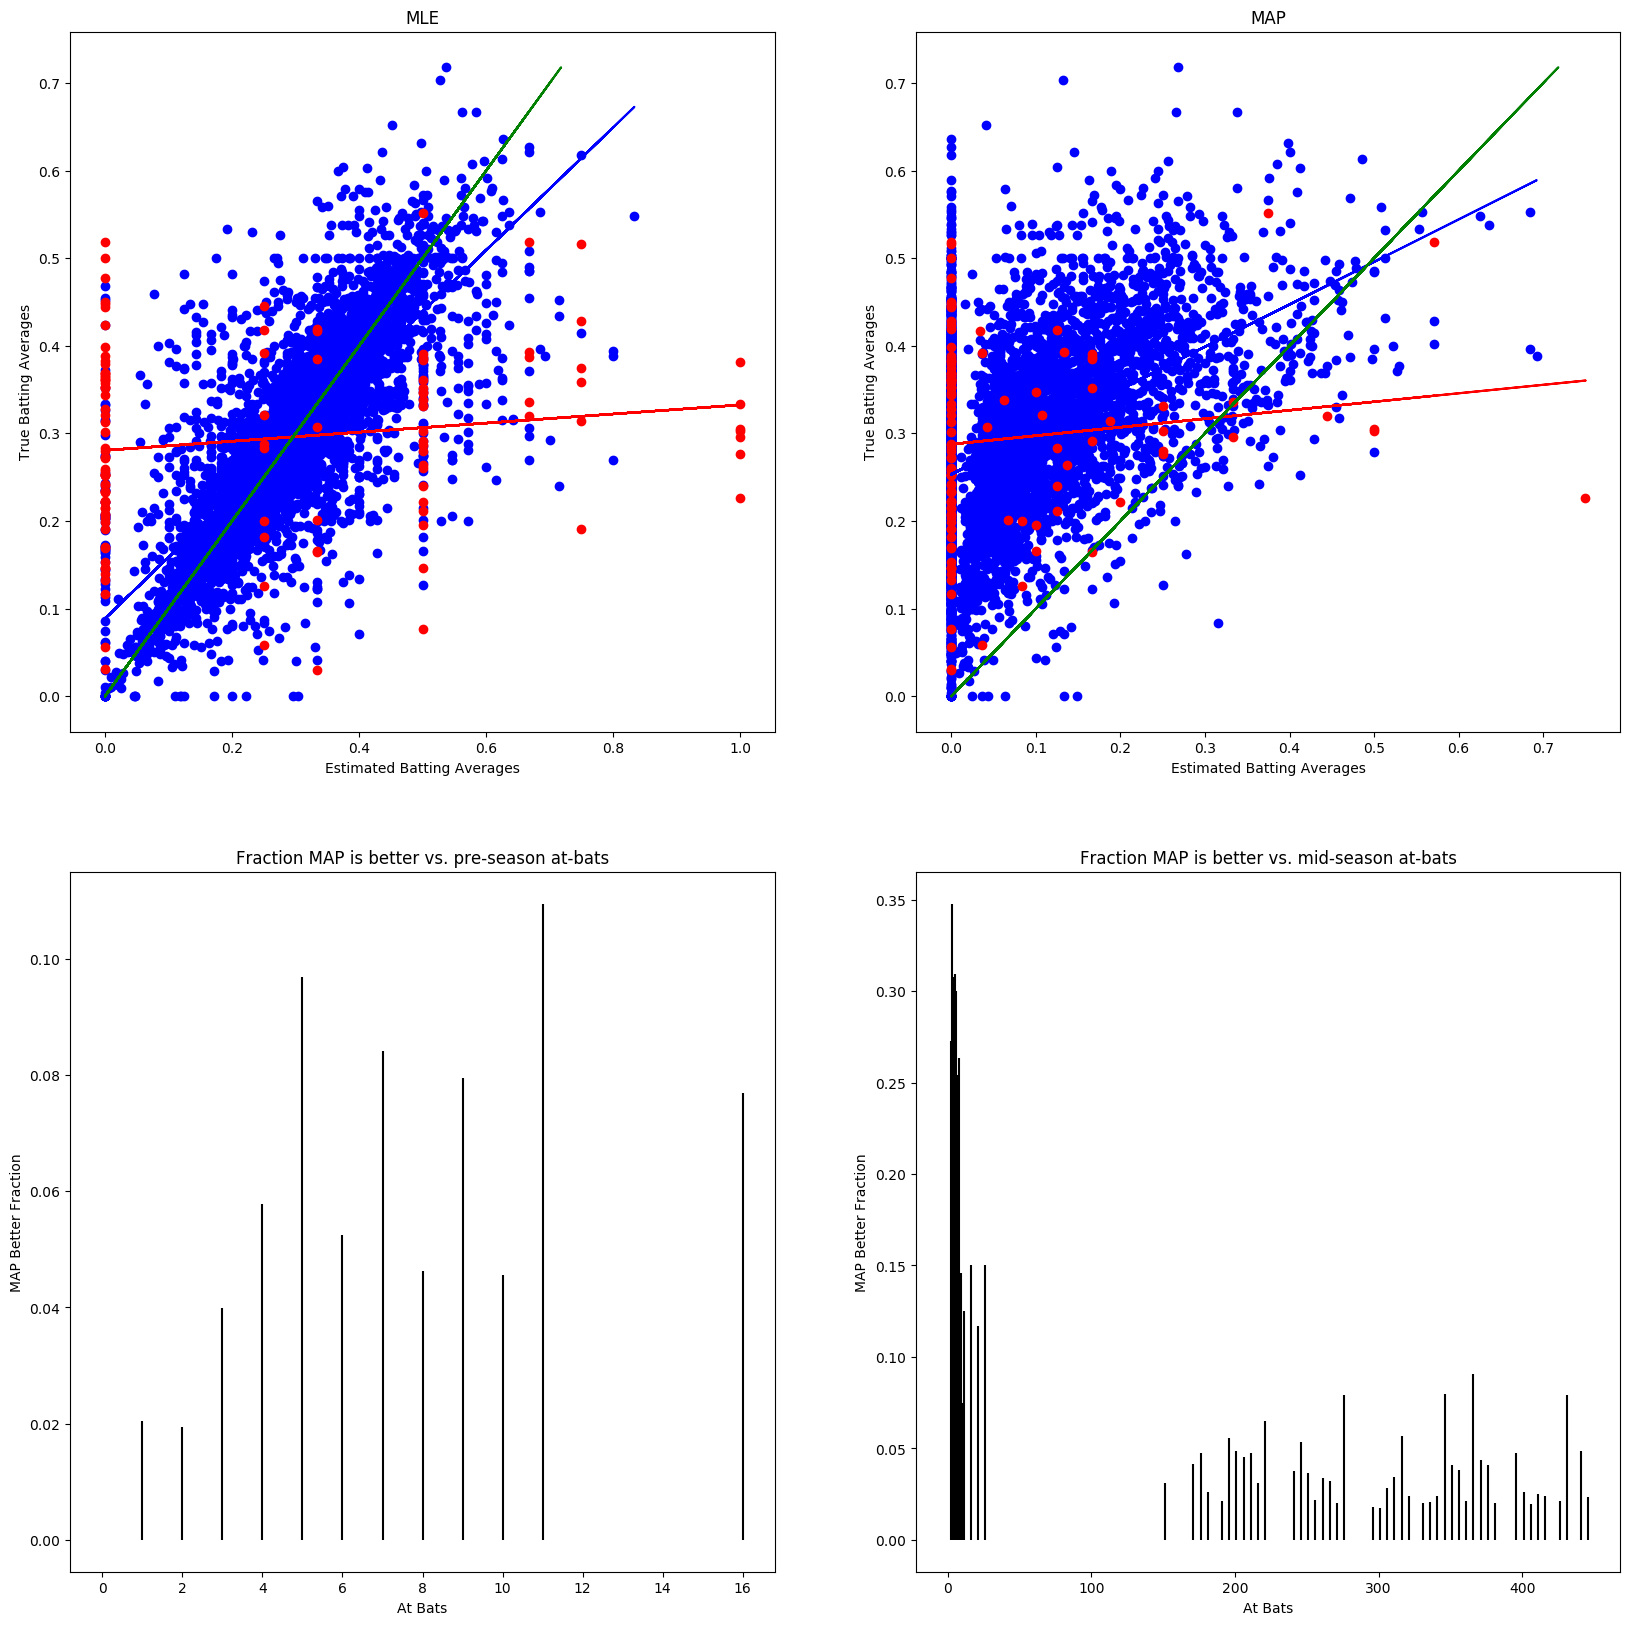
\includegraphics[width=15cm]{./Python/baseball_visualizations.png}
\end{figure}

\newpage
\subsection*{Logistic Regression on Movie Review Dataset}

In this problem, you will explore logistic regression to classify movie reviews into two classes - positive \& negative. The dataset to be used in IMDB Large Movie Review dataset (Maas et. al, ACL 2011). The datafiles are present in the link shared above.

\subsubsection*{Details about dataset}

The dataset comprises of two folders: `\textit{train}' and `\textit{test}', and each of these in turn contain two subfolders - \textit{pos} \& \textit{neg}. Each file in these subfolders is a unique review. In total, we have 25K training reviews (12.5K positive, and remaining 12.5K negative). The test folder too has 12.5K positive and 12.5K negative reviews. For our task, we will use bag of word representation.

\subsubsection*{Exercises}

For this exercise, we will directly use Logistic Regression library from \textit{sklearn.linear\_models}. We will experiment with different values of $C \in \{0.001,0.01,0.1,1,10,100\}$. Here, $C$ is the inverse of regularization constant. We will also closely study the learnt parameter/weight/coefficient vector.
\begin{itemize}
	\item Plot train and test accuracy for varying values of $C$. First plot should contain both train and test accuracy vs $C$ with $L2$ regularizer (penalty) and the second plot should employ $L1$ regularizer (penalty). What do you observe in the two plots? Which value of $C$ is optimum in these two cases?
	\\\textbf{Answer:}\\
	Fig.\ref{fig:q123}
	
	\item While using $L2$ regularizer, and different values of $C$, plot the $L2$ norm of weight vector vs $C$. What do you observe?
	\\\textbf{Answer:}\\
	Fig.\ref{fig:q123}
	
	\item While using $L1$ regularizer, and different values of $C$, plot the $L1$ norm of weight vector vs $C$. What do you observe?
	\\\textbf{Answer:}\\
	Fig.\ref{fig:q123}
	
	\begin{figure}[!h]
		\centering
		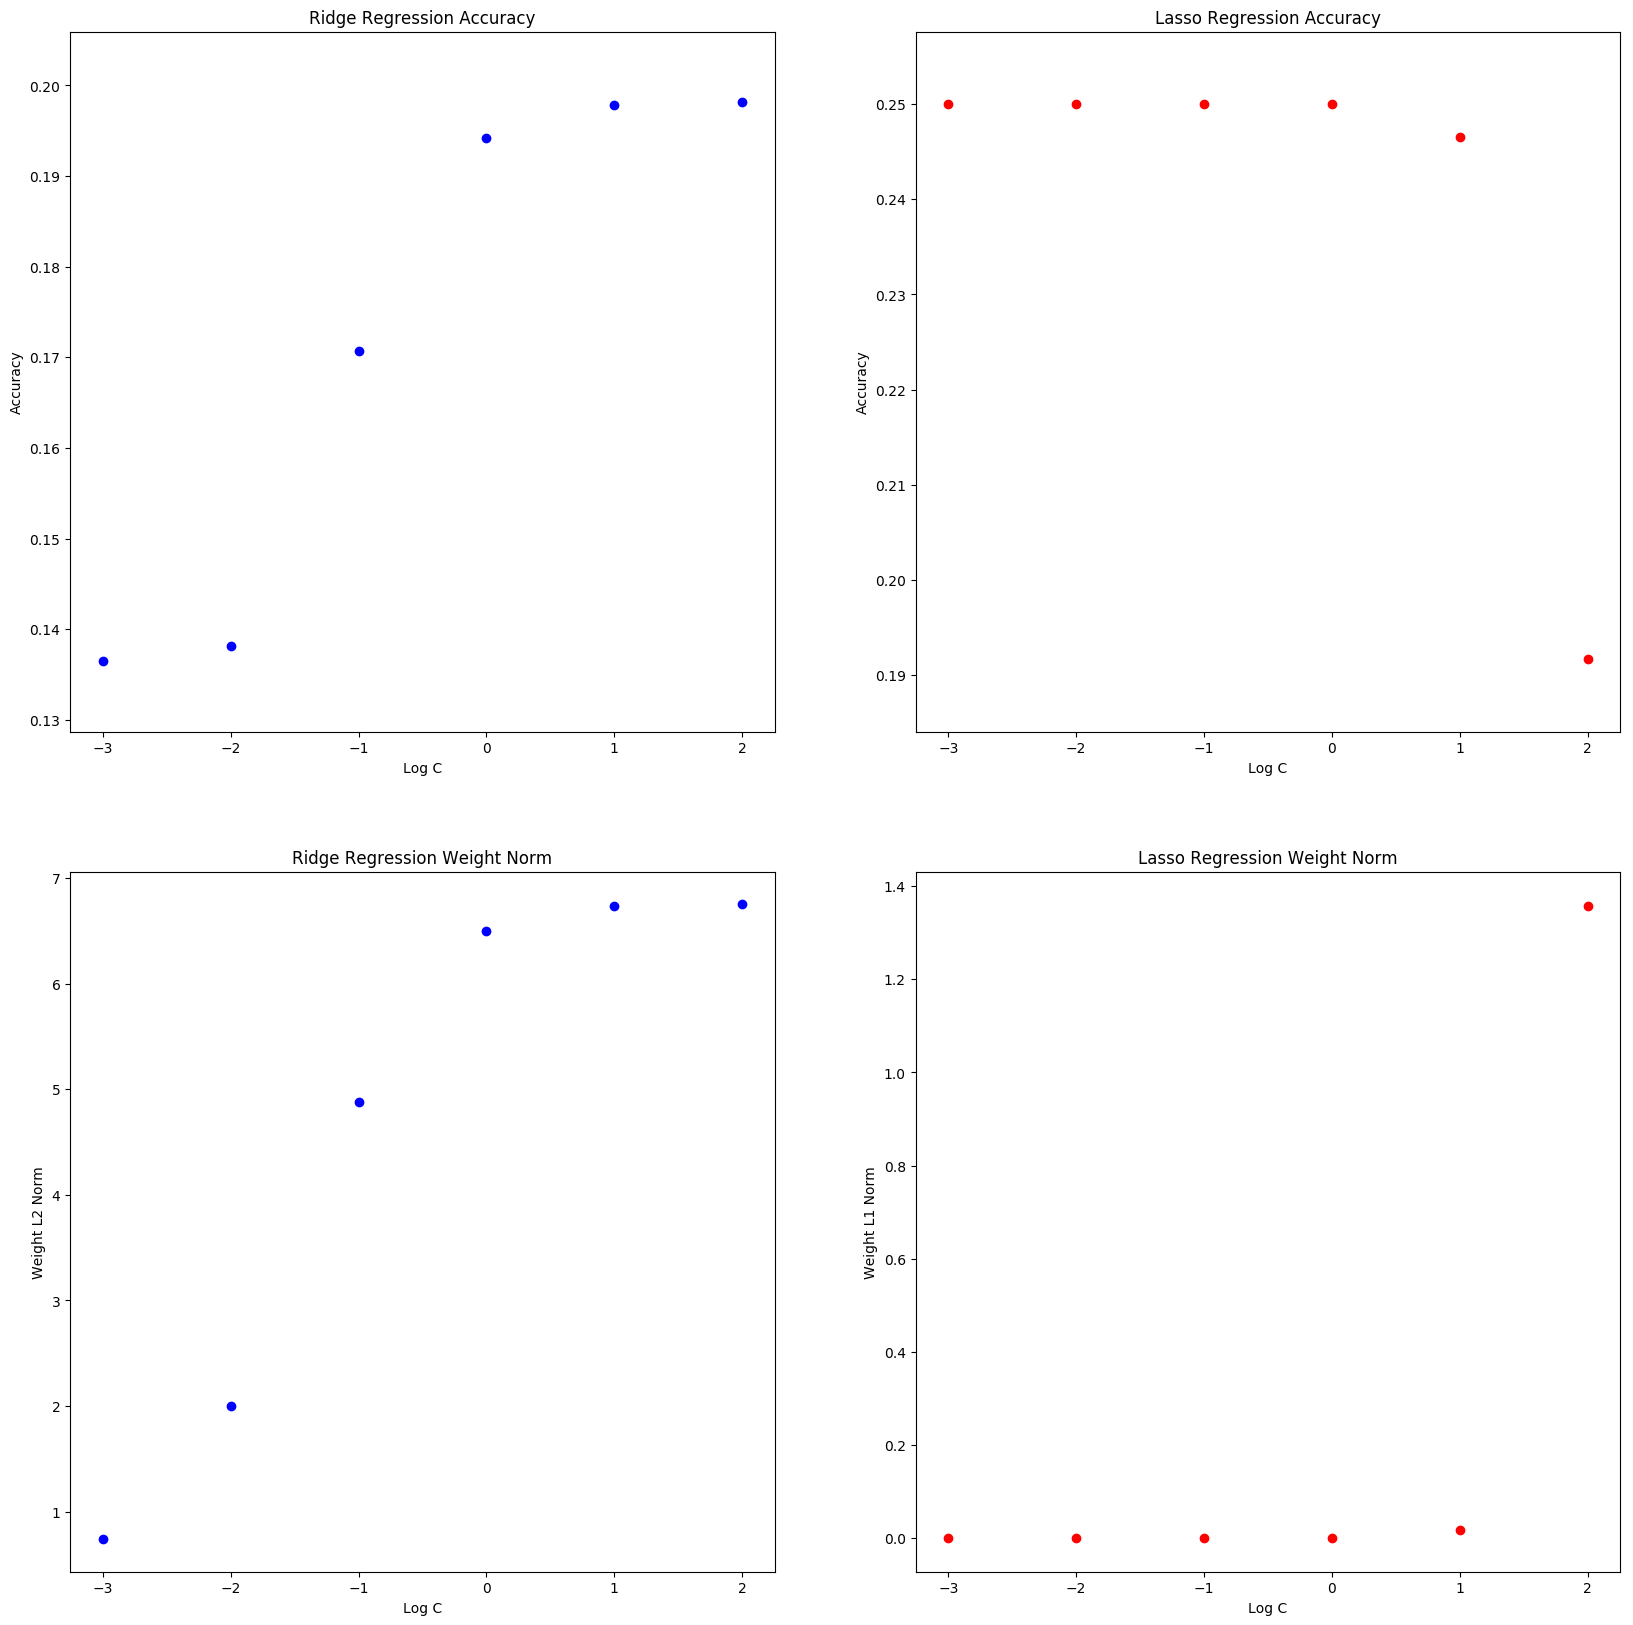
\includegraphics[width=10cm]{./Python/result1.png}
		\caption{Q1,2,3}
		\label{fig:q123}
	\end{figure}
	
	\item Study how sparsity (i.e. percentage of zero elemenets in a vector) of the parameter vector changes with different values of $C$. In one plot, depict two curves -- one for $L1$ regularizer and the other one for $L2$ regularizer. Jot down your observations.
	\\\textbf{Answer:}\\
	Fig.\ref{fig:q4}
	
	\begin{figure}[!h]
		\centering
		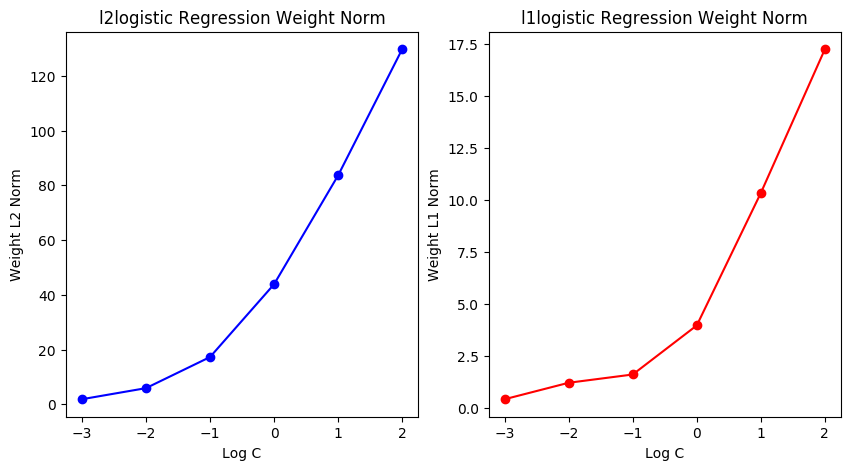
\includegraphics[width=10cm]{./Python/result2.png}
		\caption{Q4}
		\label{fig:q4}
	\end{figure}
	
\end{itemize}

Now we will try to visualize the basis of the classification! One way to do so is to look at the weight vector and analyze the top (least) $K$ values.
\begin{itemize}
	\item While using $L2$ regularizer, and the optimum value of $C$ (with respect to test accuracy), which 5 words correspond to the largest weight indices in the learnt weight vector? Which 5 words correspond to the least weight indices in the learnt parameter vector?
	\\\textbf{Answer:}\\
	\begin{itemize}
		\item Largest weight indexed words: perfect, favorite, wonderful, loved, excellent
		\item Least weight indexed words: worst, waste, awful, boring, poor
	\end{itemize}
	
	\item While using $L2$ regularizer, and the optimum value of $C$(with respect to test accuracy), which review is predicted positive with highest probability? Similary, which review is predicted negative with highest certainty?
	
	\begin{itemize}
		\item "Tony Hawk's Pro Skater 2x  isn't much different at all from the previous games  excluding Tony Hawk 3   The only thing new that is featured in Tony Hawk's Pro Skater 2x  is the new selection of levels  and tweaked out graphics  Tony Hawk's Pro Skater 2x offers a new career mode  and that is the 2x career  The 2x career is basically Tony Hawk 1 career  because there is only about five challenges per level  If you missed Tony Hawk 1 and 2  I suggest that you buy Tony Hawk's Pro Skater 2x  but if you have played the first two games  you should still try this one  Overall  there really isn't anything new  but it is still very fun to go through the game  Hopefully this review benefits your needs  Graphics  7 out of 10 Overall  the clean visuals isn't really one of Tony Hawk's Pro Skater 2x's main characteristics  The atmosphere has been changed around a lot from Tony Hawk 1 and 2  and the character models look a little bit improved  When you look back to Tony Hawk's Pro Skater 1 and 2 on the old PS1  the thought that those old graphics are ugly run through your head  In Tony Hawk's Pro Skater 2x  the graphics are rendered A LOT better  The character models are no longer filled with jaggys  the textures are more smooth  but not to the farthest extent  Tony Hawk's Pro Skater 2x's visuals do not compare to Tony Hawk 3's graphics  but Activision probably didn't want to make Tony Hawk's Pro Skater 2x have extraordinary graphics  Overall  the graphics deserve an average score of 7 because they did not put the full power of the Xbox to use in here  Graphics are nice  and clean  that's all I have to say  Sound  8 out of 10 The sound effects don't deliver much to the imagination  but the skateboards popping off of the ground sound great  The main reason why I gave the sound factor a rating  was because you are not obligated to listen to the below average Tony Hawk soundtrack  because there is a custom soundtrack feature  The sound effects sound a lot better than the sounds in Tony Hawk 1 and 2  mainly because it is more clearer  and just the fact that everything sounds great  One of the main reasons why I bought this game  is because of the custom soundtrack  The grind sound effects still sound the same as the first two games did  just a little tweaked out  One of the major problems of the sound factor  is the fact that if the song is over  it will NOT proceed to the next track  the song that you have just listened to will just play over again  I don't like the in-game soundtrack  but like I said  you are not obligated to listen to it  Controls  10 out of 10 The controls are the best part of Tony Hawk's Pro Skater 2x  The control set-up is marvelously comfortable  and easy to get used to  Back in the Playstation days  people thought that the controls were the best ever  but it looks like 2x has done a better job with the Xbox control  Surprisingly  it is very easy to use the control stick to execute tricks  Activision has done great work with Tony Hawk's Pro Skater 2x's controls  They have made the Xbox controller the best for Tony Hawk games  You will not be disappointed with the control style  and that is a guarantee  Game play  10 out of 10 Excluding the fact that Tony Hawk's Pro Skater 2x is basically Tony Hawk 1 and 2 put together  the game play is still unbelievably fun  The game play factor has been changed around a bit  This time  you get A LOT more air than in the first two games  and it is a lot easier to perform tricks  In Tony Hawk's Pro Skater 2x  each character has three career modes  consisting of Tony Hawk 1 career  Tony Hawk 2 career  and the 2x career  Tony Hawk 1 career is rather easy because in the first game  you get NOTHING for air  The Tony Hawk 2 career delivers the same amount of difficulty as the playstation version did  The only amount of difficulty that applies to the 2x career  is finding out where all items are  but after you've done that  2x career is no hard at all  In the 2x career  there is a total of 3 levels  and the first two levels consist of finding the secret tapes  collecting S-K-A-T-E  and doing whatever else is required for that particular level  The third level out of the three  is the competition level  where you have to get a certain amount of points to get the gold  In the first two levels  the secret tapes  and collecting the letters S-K-A-T-E  are featured in both of them  Overall  Tony Hawk's Pro Skater 2x still maintains the old Tony Hawk's Pro Skater vibe  Story  - Fun factor  10 out of 10 Tony Hawk's Pro Skater 2x is by far  the most funnest game on Xbox today  I have played Tony Hawk's Pro Skater 1 and 2  and back then  I didn't like them  but for some reason  Tony Hawk's Pro Skater 2x is really fun  There really isn't much to say  except that Tony Hawk's Pro Skater 2x is by far  the best game on Xbox today  One problem  is that if you've already gone through the game once  you will play it a couple more times  but it will be repetitive  Replay value  10 out of 10 Tony Hawk's Pro Skater 2x delivers a high amount of replay value  There is a lot of cheats to unlock  and a lot of character videos  Overall  Tony Hawk's Pro Skater 2x has lots of replay value  mainly because it is so fun  Best feature  You are not obligated to listen to the crappy in-game soundtrack  Worst feature  The custom soundtrack is a bit messed up  Final Statement  Lots of people have complained in the past that they didn't like Tony Hawk's Pro Skater 2x because there is nothing new  but they should stop complaining because your getting a lot of game for  50 00  Graphics  7 out of 10  Sound  8 out of 10  Control  10 out of 10  Game play  10 out of 10  Story  N A Fun factor  10 out of 10  Overall score  9 out of 10"
		\item Plankton  or Creatures from the Abyss as I'm positive it's more commonly known as   filmed under as the title Creatures from the Abyss appears over a moving image   in the same font type as the rest of the credits  starts with five 20 something kids  Mike  Clay Rogers  his girlfriend Margaret  Sharon Twomey   sisters Julie  Ann Wolf    Dorothy  Loren DePalm    an annoying idiot named Bobby  Michael Bon  whom decide to all fit into a small rubber boat   head out to sea  don't ask why as I don't know  Oh   the complete idiot Bobby left the petrol behind   never thought to tell anyone so it comes as no great surprise that they end up stranded out at sea without any petrol for the motor   to make matters worse they become trapped in a thunder storm   discover a dead body floating in the water  Shortly after their luck seems to change when they come across a yacht   potential safety  in a flash everyone boards the yacht   begin to explore  First of all they find a scientific lab with various fish specimens   computer equipment  then down below they find fully furnished   luxurious cabins  They find a chemist  Deran Sarafian  who appears mad   can't talk  They eat fish from the fridge which makes Dorothy puke up green vomit  beetles   slugs  They learn that these fish are living fossil's 1000's of years old   have been contaminated by toxic waste dumped in the sea   that they fly  mutate  bite   are generally unpleasant to be around  I really can't be bothered to go on with this plot outline so I won't  here's what I think    This Italian production was produced   directed by Massimiliano Cerchi under the pseudonym Al Passeri  I'd hide under a different name if I made a film this bad too    I think Plankton is quite simply one of the worst films ever  there are so many things wrong with this film it's difficult to know where to start  First the script by Richard Baumann is total crap  it makes no sense whatsoever   is so slow   dull it was torture for me to sit through  Why would five people just simply set sail for the middle of the ocean on a rubber dinghy barely big enough to fit them all in  What were they planning on doing exactly  Why do we often get point-of-view shots from these fish creatures but they seem to be totally invisible to the characters as they are never shown on screen even though they are right next to a character    how do these fish get around the boat as there is no water for them to swim in  People's actions   reactions to things are all wrong  they constantly split up  they make bizarre decisions that simply don't make any sense in the situation they find themselves in   some of the dialogue is as awful as anything I've heard  I could go on all day about all the plot holes   ridiculous goings on but I'll run out of space if I do  The fish creatures themselves look awful  a mixture of rubbish rubber puppets   some really bad stop motion animation at the end  the scenes where they interact with the human cast also look terrible with some bad super imposition  I have heard a lot of comments saying that Plankton is gory  don't make me laugh  Forget it there is virtually no blood or gore in Plankton whatsoever  there are a couple of slimy scenes when Bobby transforms into a fish monster while having sex with Julie but it's pretty brief   he doesn't kill her  he just sort of drips slime on her  grows a couple of tentacles   a fish head comes out of his mouth  Later on Julie's vagina starts to drip some dark slime but that's it  we never get to actually see what happens to her or what the slime is  Dorothy has a fish creature come out of her back  off screen    control her but again we never get to see what happens to her while Margaret commits suicide  a very brief shot of a plastic harpoon stuck to her forehead  Easily the grossest scene is when Dorothy pukes up that green stuff with what looks like beetles   slugs in it  That's it  only one person actually dies on screen   for the most part Plankton is quite tame   as exciting as watching paint dry   I nearly fell asleep it's so boring  I can't see how anybody can like this total crap  I just can't  The acting is awful  the dubbing is awful  the characters are awful   I hated all of them  Tecnically Plankton is predictably crap as well  with an estimated budget of only  250 000 all I can say is where did the money go  The sets are monotonous   dull with one lab   a few cabins  the special effect's are bottom of the barrel stuff including the most fake looking exploding boat ever  the cinematography is bland  the music sucks there is zero atmosphere or tension   as a whole Plankton  like it's name sake  is as low in the food chain as it could possibly be  I hate Plankton  it's awful in every single aspect of it's overlong 86 minute duration  Do yourself a favour   avoid this one at all costs unless your either a masochist or insomniac
	\end{itemize}
\end{itemize}

\end{document}
